\documentclass[a4paper,UTF8]{article}
\usepackage{ctex}
\usepackage[margin=1.25in]{geometry}
\usepackage{color}
\usepackage{graphicx}
\usepackage{amssymb}
\usepackage{amsmath}
\usepackage{amsthm}
\usepackage{enumerate}
\usepackage{bm}
\usepackage{hyperref}
\usepackage{pgfplots}
\usepackage{epsfig}
\usepackage{color}
\usepackage{tcolorbox}
\usepackage{mdframed}
\usepackage{lipsum}
\usepackage{natbib}
\usepackage{dirtree}
\usepackage{listings}
\lstset{
	columns=fixed,       
	numberstyle=\tiny\color{gray},                       % 设定行号格式
	frame=shadowbox,
	%frame=none,                                          % 不显示背景边框
	backgroundcolor=\color[RGB]{255,255,255},            % 设定背景颜色
	keywordstyle=\color[RGB]{40,40,255},                 % 设定关键字颜色
	numberstyle=\footnotesize\color{darkgray},           
	commentstyle=\it\color[RGB]{0,96,96},                % 设置代码注释的格式
	stringstyle=\rmfamily\slshape\color[RGB]{128,0,0},   % 设置字符串格式
	showstringspaces=false,                              % 不显示字符串中的空格
	language=python,                                        % 设置语言
}
\newmdtheoremenv{thm-box}{myThm}
\newmdtheoremenv{prop-box}{Proposition}
\newmdtheoremenv{def-box}{定义}

\setlength{\evensidemargin}{.25in}
\setlength{\textwidth}{6in}
\setlength{\topmargin}{-0.5in}
\setlength{\topmargin}{-0.5in}
% \setlength{\textheight}{9.5in}
%%%%%%%%%%%%%%%%%%此处用于设置页眉页脚%%%%%%%%%%%%%%%%%%
\usepackage{fancyhdr}                                
\usepackage{lastpage}                                   
\usepackage{layout}                                     
\newtheorem*{solution}{Solution}

\footskip = 10pt 
\pagestyle{fancy}                    % 设置页眉                 
\lhead{2020年秋季}                    
\chead{高级机器学习}                                                
% \rhead{第\thepage/\pageref{LastPage}页} 
\rhead{作业二}                                                                                               
\cfoot{\thepage}                                                
\renewcommand{\headrulewidth}{1pt}  			%页眉线宽,设为0可以去页眉线
\setlength{\skip\footins}{0.5cm}    			%脚注与正文的距离           
\renewcommand{\footrulewidth}{0pt}  			%页脚线宽,设为0可以去页脚线

\makeatletter 									%设置双线页眉                                        
\def\headrule{{\if@fancyplain\let\headrulewidth\plainheadrulewidth\fi%
\hrule\@height 1.0pt \@width\headwidth\vskip1pt	%上面线为1pt粗  
\hrule\@height 0.5pt\@width\headwidth  			%下面0.5pt粗            
\vskip-2\headrulewidth\vskip-1pt}      			%两条线的距离1pt        
 \vspace{6mm}}     								%双线与下面正文之间的垂直间距              
\makeatother  

%%%%%%%%%%%%%%%%%%%%%%%%%%%%%%%%%%%%%%%%%%%%%%
\numberwithin{equation}{section}
%\usepackage[thmmarks, amsmath, thref]{ntheorem}
\newtheorem{myThm}{myThm}
\newtheorem*{myDef}{Definition}
\newtheorem*{mySol}{Solution}
\newtheorem*{myProof}{Proof}
\newtheorem*{myRemark}{备注}
\renewcommand{\tilde}{\widetilde}
\renewcommand{\hat}{\widehat}
\newcommand{\indep}{\rotatebox[origin=c]{90}{$\models$}}
\newcommand*\diff{\mathop{}\!\mathrm{d}}

\usepackage{multirow}

%--

%--
\begin{document}
\title{高级机器学习\\
大作业}
\author{周韧哲\,181220076} 
\maketitle
%%%%%%%% 注意: 使用XeLatex 编译可能会报错,请使用 pdfLaTex 编译 %%%%%%%

\section*{学术诚信}

本课程非常重视学术诚信规范,助教老师和助教同学将不遗余力地维护作业中的学术诚信规范的建立。希望所有选课学生能够对此予以重视。\footnote{参考尹一通老师\href{http://tcs.nju.edu.cn/wiki/}{高级算法课程}中对学术诚信的说明。}

\begin{tcolorbox}
	\begin{enumerate}
		\item[(1)] 允许同学之间的相互讨论,但是{\color{red}\textbf{署你名字的工作必须由你完成}},不允许直接照搬任何已有的材料,必须独立完成作业的书写过程;
		\item[(2)] 在完成作业过程中,对他人工作(出版物、互联网资料)中文本的直接照搬(包括原文的直接复制粘贴及语句的简单修改等)都将视为剽窃,剽窃者成绩将被取消。{\color{red}\textbf{对于完成作业中有关键作用的公开资料,应予以明显引用}};
		\item[(3)] 如果发现作业之间高度相似将被判定为互相抄袭行为,{\color{red}\textbf{抄袭和被抄袭双方的成绩都将被取消}}。因此请主动防止自己的作业被他人抄袭。
	\end{enumerate}
\end{tcolorbox}

\section*{作业提交注意事项}
\begin{tcolorbox}
	\begin{enumerate}
		\item[(1)] 请在LaTeX模板中{\color{red}\textbf{第一页填写个人的姓名、学号信息}};
		\item[(2)] 本次作业需提交该pdf文件、直接可以运行的源码,将以上几个文件压缩成zip文件后上传。zip文件格式为{\color{red}\textbf{学号.zip}},例如170000001.zip;pdf文件格式为{\color{red}\textbf{学号\_姓名.pdf}},例如170000001\_张三.pdf。
		\item[(3)] 未按照要求提交作业,或提交作业格式不正确,将会{\color{red}\textbf{被扣除部分作业分数}};
		\item[(4)] 本次作业提交截止时间为{\color{red}\textbf{1月8日23:59:59}}。除非有特殊情况(如因病缓交),否则截止时间后不接收作业,本次作业记零分。
	\end{enumerate}
\end{tcolorbox}

\newpage
\section{Introduction}
本次的作业为使用条件随机场(conditional random field,CRF)解决OCR(optical character recognition)问题。

在CRF模型中,有两种变量:我们要建模的隐藏变量和始终观察到的变量。对于OCR,我们要在观察的字符图像(也就是每个图像对应的像素数组)的情况下,对字符(例如“a”或“c”)进行建模。通常来说,未观察到的变量用$Y$表示,观察到的变量用$X$表示。CRF试图对$P(Y|X)$建模,即给定观察到的图像上字符的条件分布。该模型的结构如\ref{Fig.main1}下所示:
\begin{figure}[h] 
\centering
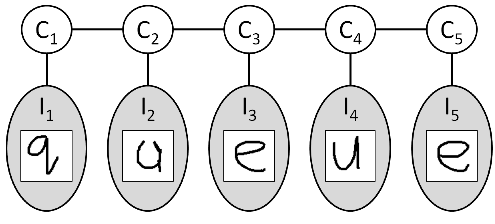
\includegraphics[width=0.7\textwidth]{figs/fig1.png} 
\caption{Markov Network} 
\label{Fig.main1}
\end{figure}

在CRF中,每个特征都对应一个权重$\theta_i$,在给定特征和权重的情况下,条件概率分布可以表示为:
\begin{equation}
P(\mathbf{Y} \mid \mathbf{x}: \theta)=\frac{1}{Z_{\mathbf{x}}(\theta)} \exp \left\{\sum_{i=1}^{k} \theta_{i} f_{i}\left(\mathbf{Y}, \mathbf{x}\right)\right\}\label{eq1}
\end{equation}

其中,$Z_x(\theta)$为配方函数
\begin{equation}
Z_{\mathbf{x}}(\theta) \equiv \sum_{\mathbf{Y}} \exp \left\{\sum_{i=1}^{k} \theta_{i} f_{i}\left(\mathbf{Y}, \mathbf{x}\right)\right\}
\end{equation}

在这次的任务中,一共有三类特征,三类特征均为指示函数,即满足条件时$f=1$,不满足时$f=0$:
\begin{itemize}
    \item $f_{i, c}^{C}\left(Y_{i}\right)$,指示是否$Y_i = c$
    \item $f_{i, j, c, d}^{I}\left(Y_{i}, x_{i j}\right)$,指示是否$Y_i=c,x_{ij}=d$
    \item $f_{i, c, d}^{P}\left(Y_{i}, Y_{i+1}\right)$,指示是否$Y_i=c,Y_{i+1}=d$
\end{itemize}

建立好模型,给定训练样本,我们就可以使用最大似然估计来进行学习:
\begin{equation}
    LL(\mathbf{x},\mathbf{Y},\theta) =\sum_{i=1}^{k} \theta_{i} f_{i}(\mathbf{Y}, \mathbf{x}) -\log \left(Z_{\mathbf{x}}(\theta)\right)\label{eq2}
\end{equation}

对于这个目标,我们可以使用梯度上升算法学习参数。

\section{Dataset}
本题中的数据集一共包含两个部分\texttt{trainset}和\texttt{testset}, 分别是训练集和测试集.训练集中有400个样本,测试集中有200个样本. 每个样本被存储在一个\texttt{txt}文件中, 第一行为对应的单词, 之后的每行为单词的每个字母对应的像素的状态.

\section{Assignment}
\begin{enumerate}
    \item 建立CRF模型,在训练集上进行训练,使用梯度上升的方法对模型参数进行求解,即求解公式\eqref{eq2}(注:不允许使用现有的CRF包,使用python实现)。
    \item 在模型训练完成后,在测试集上进行推断,评价模型的性能。
    \item 使用一些其他方法提高模型性能,可参考以下几个方面但不限于此:
    \begin{itemize}
        \item 提高模型表达能力:如在CRF图上添加新的连接。
        \item 缓解模型过拟合:如添加正则项。
        \item 加速模型训练过程:如权重共享。
    \end{itemize}
    \item 完成实验报告,主要包含具体的实现方法,如何复现运行代码,对模型的改进以及结果的分析等部分。
\end{enumerate}
\section {实验报告}
\subsection{项目运行}
本repo的目录树如下:

\begin{minipage}{\linewidth}
\dirtree{%
	.1 \textcolor{cyan}{HW3}.
	.2 \textcolor{cyan}{model}.
	.3 graph.py.
	.3 linear\_chain\_crf.py.
	.2 \textcolor{cyan}{utils}.
	.3 trainer.py.
	.3 utils.py.
	.2 train\_crf.py.
}
\end{minipage}

模块graph为图模型的基类实现,模块linear\_chain\_crf中为线性链条件随机场的实现,继承了Graph;trainer为训练模块的集成,将模型的实现与训练解耦;模块utils里为数据的加载及其处理;train\_crf为代码运行的script,集成了加载、训练与测试的过程。train\_crf.py中可选命令行参数有种子seed,学习率lr,批数据大小batch\_size,训练轮数epoch,正则项系数lamda,特征中共享变量的特征数shared\_nums等等。在本repo的根目录下命令行键入python train\_crf.py会按默认参数运行,会得到一个在测试集上正确率为0.998的结果。下面我将会介绍我的具体实现与模型改进和对比的结果。
\subsection{具体实现}
数据的观察序列的维度为321维,状态一共有10种。对于题目所给的三类特征C、I、P,实际上可以分为状态特征C和I与转移特征P。因为状态特征只和当前时间有关,转移特征和当前时间以及下一个时间有关,这样的考虑可以减少变量,简化实现。
\subsubsection{加载数据}
数据加载实现在utils/utils.py中,load\_data函数会直接将原来的320维像素(不考虑第一维是因为它全为1)作为CRF的特征,即上面提到的特征I,而load\_data\_c则会加上特征C,即考虑每个时间位置的标签类型,因而要比原特征多10个维度,实验显示加入这个特征可以提升泛化性能。
\subsubsection{CRF模型}
在model/graph.py中我定义了一个抽象类Graph,在其中初始化了特征参数thetaP和thetaI,并定义了一系列方法。LinearChainCRF继承了类Graph。实现CRF需要计算配分函数Z,完全遍历的计算会导致组合爆炸问题,因此我使用了信念传播算法来通过传递消息来快速计算边际概率,对应compute\_message函数。链式CRF的消息传递分为前向和后向,即从序列开头和结尾开始传递的消息。首先初始化消息为1,然后从左到右计算每一个团之间的消息,在当前时刻,它需要向右传递的消息是它接收到的消息乘以此时刻的势函数。在实现中我将势函数按特征分开,在基类中的两个property potP和potI就是对应特征的势函数。
compute\_fweight函数是计算特征和权重的乘积和,即$\sum_k^K \theta_k f_k$。如此便可以计算出对数似然
$\sum_{k=1}^{K} \theta_{k} f_{k}(\mathbf{Y}, \mathbf{x}) -\log \left(Z_{\mathbf{x}}(\theta)\right)$,对应于compute\_ll函数。

完成消息传递后就能够计算每个位置的边际分布$P(Y_i|X)$和成对分布$P(Y_i,Y_{i+1}|X)$,分别对应compute\_marginal\_dist和compute\_pair\_dist。从而可以在该CRF模型上进行推理:从初始时刻开始,第一个位置被预测为$\arg\max _i P_1(Y_i|X)$,由于我们知道了接下来时刻位置的边际分布和成对分布,在第t-1个时刻位置被预测为$y_{t-1}$的情况下,第t个时刻位置将会被预测为$\arg\max_i P_{t-1}(y_{t-1},Y_i|X)P_t(Y_i|X)$。

令序列长度为K,特征数记为F,标签数记为M,给定了参数thetaI($M\times F$)和thetaP($M\times M$)下,为了计算导数,首先将其对数似然函数展开:
\begin{align*}
	LL(X,Y,\theta_I,\theta_P) &= \sum_{i=1}^K\sum_{f=1}^F\theta^I_{y_i,f}X_{if}+ \sum_{i=1}^{K-1}\theta^P_{y_iy_{i+1}}\times 1-\log Z
\end{align*}
对thetaP求导得
\begin{align*}
	\frac{\partial LL}{\partial \theta^P_{y',y\_}} &=\sum_{i=1}^{K-1}\frac{\partial \theta^P_{y_i,y_{i+1}} }{\partial \theta^P_{y',y\_}}-\frac{1}{Z}\frac{\partial}{\partial \theta^I_{y',y\_}}\sum_y\exp(\sum_{i=1}^{K}\sum_{f=1}^F\theta^I_{y_i,f}X_{if}+ \sum_{i=1}^{K-1}\theta^P_{y_iy_{i+1}}\times 1)\\
	&=\sum_{i=1}^{K-1}\mathbb{I}[y_i=y',y_{i+1}=y\_]-\frac{1}{Z}\frac{\partial}{\partial \theta^I_{y',y\_}}\sum_y\exp(\sum_{i=1}^{K-1}\theta^P_{y_iy_{i+1}}\times 1)\mathbb{I}[y_i=y',y_{i+1}=y\_]\\
	&=\sum_{i=1}^{K-1}\mathbb{I}[y_i=y',y_{i+1}=y\_]-\sum_y P(y|X)\mathbb{I}[y_i=y',y_{i+1}=y\_]
\end{align*}
对thetaI求导得
\begin{align*}
	\frac{\partial LL}{\partial \theta^I_{y',f'}} &=\sum_{i=1}^K\sum_{f=1}^F\frac{\partial \theta^I_{y_i,f}}{\partial \theta^I_{y',f'}}X_{if}-\frac{1}{Z}\frac{\partial}{\partial \theta^I_{y',f'}}\sum_y\exp(\sum_{i=1}^K\sum_{f=1}^F\theta^I_{y_i,f}X_{if}+ \sum_{i=1}^{K-1}\theta^P_{y_iy_{i+1}}\times 1)\\
	&=\sum_{i=1}^K\sum_{f=1}^F\mathbb{I}[y_i=y',f=f']X_{if}-\frac{1}{Z}\frac{\partial }{\partial \theta^I_{y',f'}}\sum_y\exp(\sum_{i=1}^K\sum_{f=1}^F\theta^I_{y_i,f}X_{if}+ \sum_{i=1}^{K-1}\theta^P_{y_iy_{i+1}}\times 1)\\
	&=\sum_{i=1}^K\sum_{f=1}^F\mathbb{I}[y_i=y',f=f']X_{if}-\frac{1}{Z}\frac{\partial}{\partial \theta^I_{y',f'}}\sum_y\exp(\sum_{i=1}^K\sum_{f=1}^F\theta^I_{y_i,f}X_{if}+ \sum_{i=1}^{K-1}\theta^P_{y_iy_{i+1}}\times 1)\\
	&\qquad\qquad\qquad\qquad\qquad\qquad\qquad\qquad\qquad\qquad\qquad\qquad\qquad\times \mathbb{I}[y_i=y',f=f']X_{if}\\
	&=\sum_{i=1}^K\sum_{f=1}^F\mathbb{I}[y_i=y',f=f']X_{if}-\sum_y P(y|X)\mathbb{I}[y_i=y',f=f']X_{if}
\end{align*}
详见commpute\_grad函数。在实现中我也加入了L2正则项$\frac{\lambda}{2}\|\theta\|_2^2$,其导数就是$\lambda\theta$,因此只需让上面的梯度加上$\lambda \theta$即可。
\subsubsection{训练与测试}
在trainer模块中实现了一个用于管理训练过程的类Trainer,其函数train实现了批量梯度上升,在每个epoch中,先把训练集打乱,然后计算batch\_size个训练样本对的平均梯度用于梯度上升。每完成一个epoch后,就会计算当前的目标函数值,即对数似然值,并在测试集上推断,打印出accuracy。训练完成后,会打印出运行时间。
\subsection{实验结果与总结}
我做了以下几个实验来探讨模型的不同改进点的性能差异。
\subsubsection{权重共享}
不同的权重共享对模型的影响。对于图片的320个像素值,设权重共享数为k,则每k个共享一个权值,表\ref{table1}是当k为1,4,8,16,20时的运行时间表,每个运行了5次,epoch为100,随机种子固定为0,学习率为0.01,batch\_size为16,正则化系数$\lambda$为0,都使用了C特征,因而维度要多出10维,其对应的权重矩阵维度分别为330,90,50,30,26。由表可知,这几种情况的运行时间相差不大,最长的仅比最短的多3秒左右,而共享权重数越大时,性能越不好,见图\ref{figure1},横轴为迭代次数,纵轴分别为Accuracy和LogLikeliHood。当k为1和4时准确率都达到了0.99,且它们在较短的迭代次数内就到达了一个较高的准确率。
\begin{table}
\caption{权重共享(单位:秒),CPU:Intel Core i5-9300HF}
\label{table1}
\begin{center}
\begin{tabular}{|c|c|c|c|c|c|}
	\hline
	shared\_nums& 1& 4 &8 & 16 & 20\\
	\hline
	mean & 14.05& 12.41 & 11.92& 11.31& 11.45\\
	\hline
	std & 0.68& 0.24& 0.36 & 0.41& 0.39\\
	\hline
\end{tabular}
\end{center}
\end{table}

\begin{figure}[h] 
	\centering
	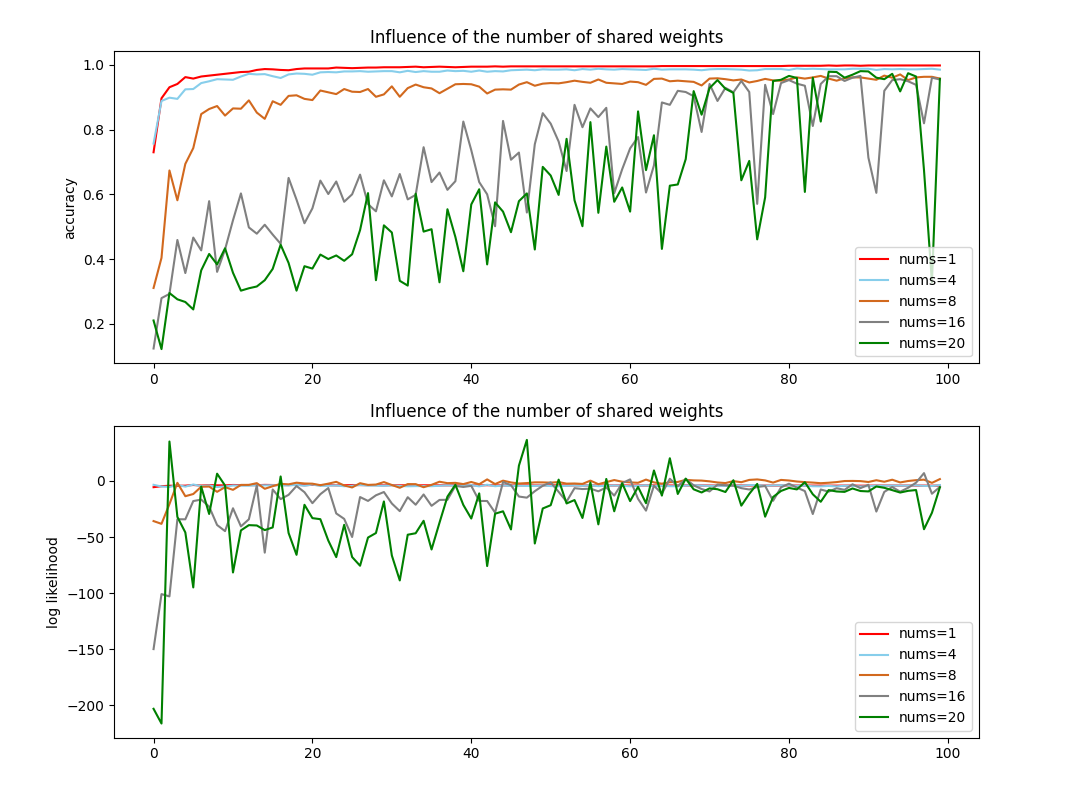
\includegraphics[width=0.8\textwidth]{figs/Figure_1.png} 
	\caption{Shared nums} 
	\label{figure1}
\end{figure}
\subsubsection{正则化}
我测试了5种不同的正则化系数$\lambda$为0,0.005,0.05,0.5,5,权重共享数为1,其他实验设置与上一小节一致,见图\ref{figure2},横轴为迭代次数,纵轴分别为Accuracy和LogLikeliHood,发现正则化系数较小时并没有太大的变化,而较大时会导致模型欠拟合,效果不佳。我认为是因为这个任务的特征提取得比较好,模型比较容易学,因而正则化不会导致太大的作用,并且在没有正则化时,模型的泛化性能已经很好了。

\subsubsection{使用特征C}
最后我探讨了使用特征C与否造成的影响,设置正则化系数为0,其他实验设置与上一小节一致,在train\_crf.py中可以通过命令行参数not\_use\_c来控制是否使用特征C。由图\ref{figure3}容易看出,加入特征C提高了模型在测试集上的最高准确率,对泛化性能有较不错的提升。因为特征C指示了当前处于哪种状态,而在英语中不同字母在单词的不同位置出现的概率是不一样的,将这一特征加入可以让模型学得更好。

\begin{figure}[h] 
	\centering
	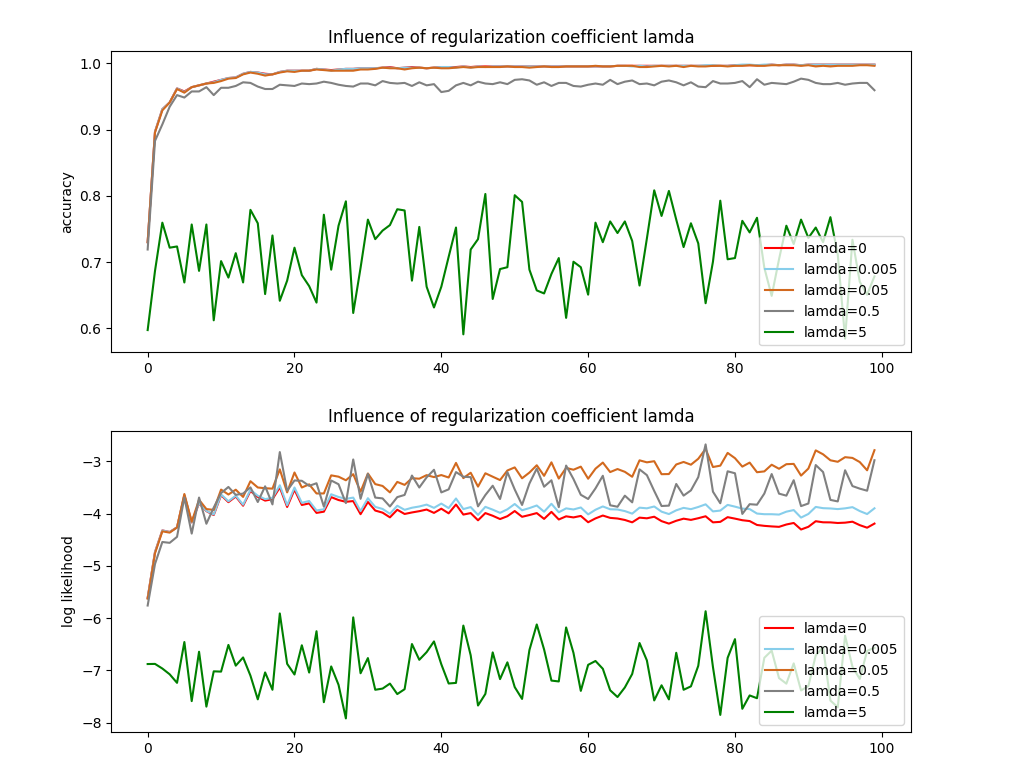
\includegraphics[width=0.8\textwidth]{figs/Figure_2.png} 
	\caption{Regulariation} 
	\label{figure2}
\end{figure}
\begin{figure}[h] 
	\centering
	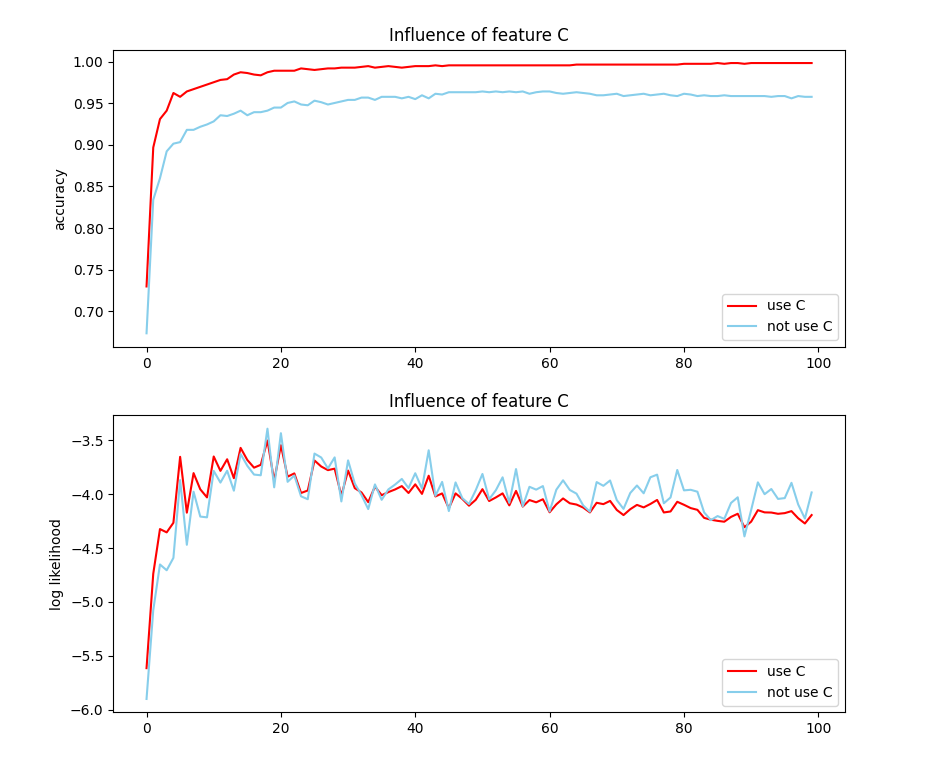
\includegraphics[width=0.8\textwidth]{figs/Figure_3.png} 
	\caption{特征C} 
	\label{figure3}
\end{figure}
\subsubsection{实验总结}
用条件随机场做此任务十分合适,因为单词是不定长序列,且是有时序位置关系的,因而模型能取得很好的效果。难点在于构建特征和消息传播算法,如果单词长度短的话,直接遍历所有可能序列是在时间上可以接受的,但这次任务的数据集中存在8、9个字母的单词,遍历会导致时间复杂度很高,运行时间很长。

最后,祝助教学长和老师新年快乐!
\end{document}